\documentclass{emulateapj}
\submitted{{\it Submitted for publication in ApJL}}
\usepackage{multirow,color,wrapfig,ulem}
\usepackage {graphicx}

\usepackage{graphics}
\usepackage[dvips]{epsfig}

\newcommand{\avg}[1]{\langle{#1}\rangle}  
\newcommand{\nscatt}{\langle N_{\rm  scatt}\rangle}
\newcommand{\ly}{{\ifmmode{{\rm Ly}\alpha~}\else{Ly$\alpha$~}\fi}}
\newcommand{\hMpc}{{\ifmmode{h^{-1}{\rm Mpc}}\else{$h^{-1}$Mpc }\fi}}   
\newcommand{\hGpc}{{\ifmmode{h^{-1}{\rm Gpc}}\else{$h^{-1}$Gpc }\fi}}   
\newcommand{\hmpc}{{\ifmmode{h^{-1}{\rm Mpc}}\else{$h^{-1}$Mpc }\fi}}  
\newcommand{\hkpc}{{\ifmmode{h^{-1}{\rm kpc}}\else{$h^{-1}$kpc }\fi}}  
\newcommand{\hMsun}{{\ifmmode{h^{-1}{\rm
        {M_{\odot}}}}\else{$h^{-1}{\rm{M_{\odot}}}$}\fi}}   
\newcommand{\hmsun}{{\ifmmode{h^{-1}{\rm
        {M_{\odot}}}}\else{$h^{-1}{\rm{M_{\odot}}}$}\fi}}   
\newcommand{\Msun}{{\ifmmode{{\rm {M_{\odot}}}}\else{${\rm{M_{\odot}}}$}\fi}}  
\newcommand{\msun}{{\ifmmode{{\rm {M_{\odot}}}}\else{${\rm{M_{\odot}}}$}\fi}}  
\newcommand{\lya}{{Lyman$\alpha$~}}
\newcommand{\clara}{{\texttt{CLARA}}~}
\newcommand{\rand}{{\ifmmode{{\mathcal{R}}}\else{${\mathcal{R}}$ }\fi}}  
\newcommand{\hs}{{\hspace{1mm}}}  
\newcommand{\kms}{{\ifmmode{{\mathrm{\,km\ s}^{-1}}}\else{\,km~s$^{-1}$}\fi}}

% definition to produce a "less than or similar to" symbol
\def\lsim{~\rlap{$<$}{\lower 1.0ex\hbox{$\sim$}}}

% definition to produce a "greater than or similar to" symbol
\def\gsim{~\rlap{$>$}{\lower 1.0ex\hbox{$\sim$}}}

\begin{document}

\title{Cosmic Web} 
\author{
  XXXX\altaffilmark{1},
  YYYY\altaffilmark{2},
  ZZZZ\altaffilmark{3}
}

\altaffiltext{1}{Uni A}
\altaffiltext{2}{Uni B}
\altaffiltext{3}{Uni C}
\begin{abstract}
This
\end{abstract}

\begin{keywords}
{galaxies: high-redshift,galaxies: star formation, line: formation}
\end{keywords}


\section{Introduction}
\label{sec:intro}

\section{Simulation and web finding algorithm}
\label{sec:Simulation}

\section{Results}
\label{sec:results}

\citep{Hillier98}


\begin{table}
\begin{center}
\begin{tabular}{lcccc}\hline\hline
Sample & Peak & Filament & Sheet & Void\\
       & $n$ (\%) & $n$ (\%) & $n$ (\%) & $n$ (\%) \\\hline
2$\sigma$ & 10 (8.1) & 59 (48.3) & 48 (39.3) & 5 (4.0)\\  
3$\sigma$ & 4 (8.5) & 24 (51.0) &  18 (38.2) & 1 (2.1)\\
General & 1307 (23.8) & 1470 (26.8) & 1769 (32.3) & 927 (16.9)\\\hline
\end{tabular}
\caption{
Number of pairs in the four different kinds of environmtns. In
parethesis the same number as a percentage of the
total population. 
\label{table:models}}
\end{center}
\end{table}

\begin{table}
\begin{center}
\begin{tabular}{lccc}\hline\hline
Sample & $\langle\hat{e}_1\cdot \hat{n}\rangle$ & $\langle\hat{e}_2\cdot \hat{n}\rangle$ & $\langle\hat{e}_3\cdot \hat{n}\rangle$\\\hline
2$\sigma$ & 0.56 & 0.53 &  0.33\\
3$\sigma$ & 0.51 & 0.51 &  0.46\\
General & 0.54 & 0.52 & 0.40\\\hline
\end{tabular}
\caption{Average values for the cosinus between the three eigenvectors and the vector normal to the orbital plane.
\label{table:mu}}
\end{center}
\end{table}


\begin{figure}
\begin{center}
  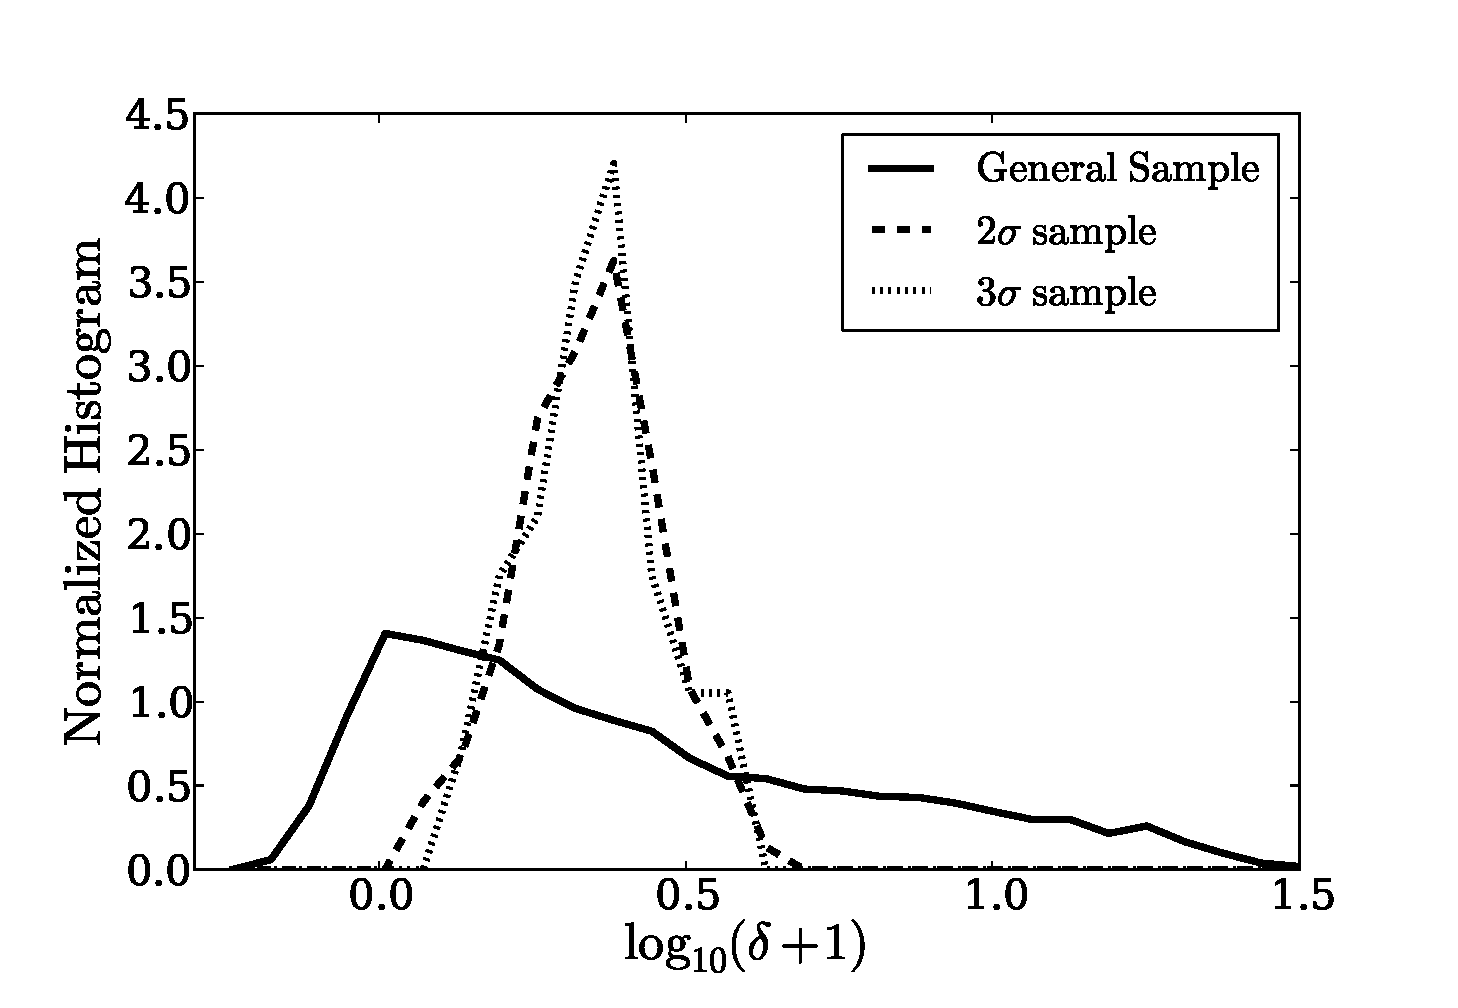
\includegraphics[width=0.45\textwidth]{density_histogram.eps}
\end{center}
\caption{Overdensity distribution for the pairs in the three samples.
    \label{fig:density}}  
\end{figure}


\begin{figure}
\begin{center}
  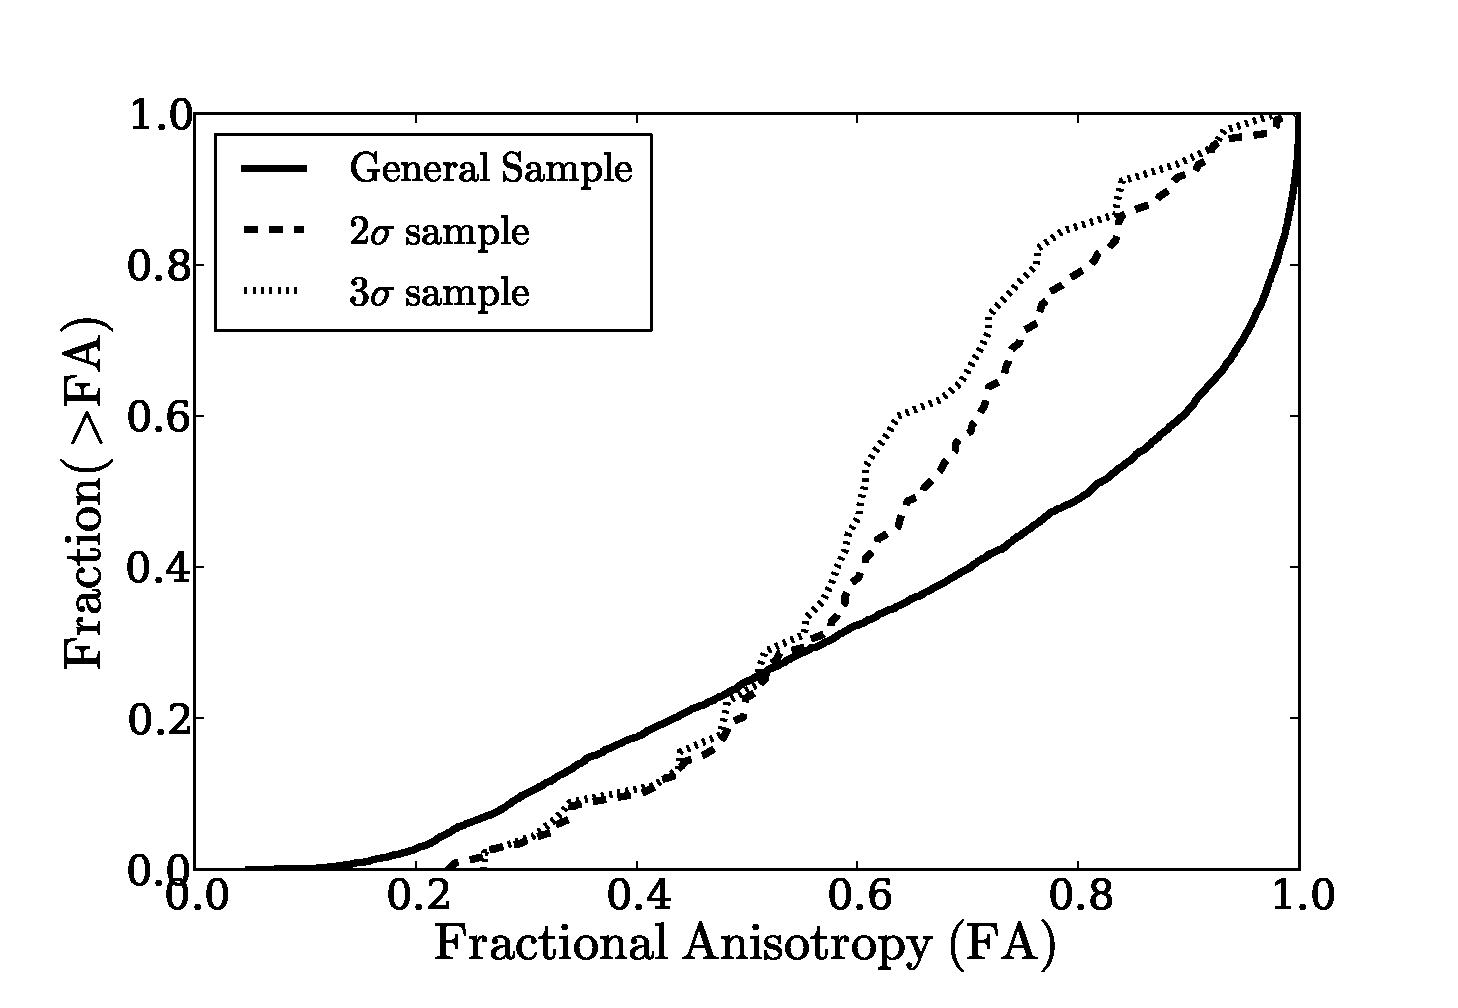
\includegraphics[width=0.45\textwidth]{FA_histogram.eps}
\end{center}
\caption{Integrated Fractional Anisotropy distribution for the pairs in the three samples.
    \label{fig:FA}}  
\end{figure}

\begin{figure}
\begin{center}
  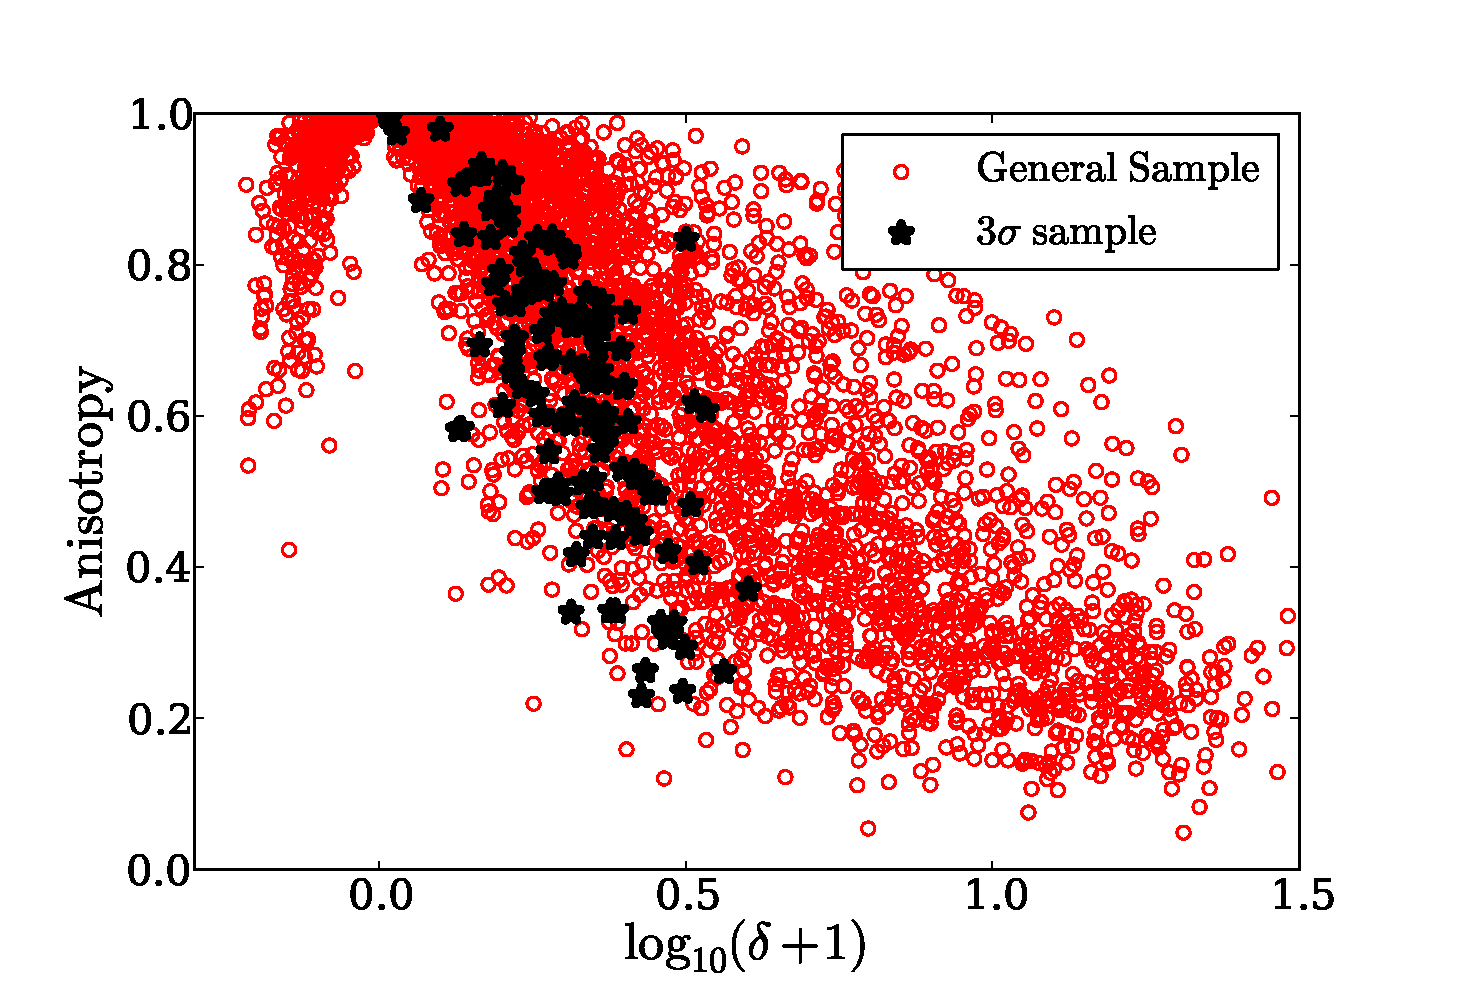
\includegraphics[width=0.45\textwidth]{FA_delta_scatter.eps}
\end{center}
\caption{Density and Fractional Anisotropy distribution for the pairs in the general and $3\sigma$ samples.
    \label{fig:FA}}  
\end{figure}

\section{Discussion}
\label{sec:discussion}

\section{Conclusions}
\label{sec:conclusions}


\section*{Acknowledgements}

\bibliographystyle{apj}
\bibliography{references} 


\end{document}


